\documentclass[a4paper]{article}
\usepackage[utf8]{inputenc}
\usepackage[T1]{fontenc}
\usepackage[light,condensed,math]{kurier}
\usepackage[ngerman]{babel}
\usepackage{ntheorem}
\usepackage{graphicx}
\usepackage{floatrow}
\usepackage{float}
\usepackage{hyperref}
\usepackage{mathtools}
\usepackage{amssymb}
\usepackage{minted}

\theoremstyle{break}

\usepackage{titlesec}
\setcounter{secnumdepth}{4}
\titleformat{\paragraph}
{\normalfont\normalsize\bfseries}{\theparagraph}{1em}{}
\titlespacing*{\paragraph}
{0pt}{3.25ex plus 1ex minus .2ex}{1.5ex plus .2ex}

\newtheorem{formula}{Formel}[section]
\newtheorem{defi}{Definition}[section]
\newtheorem{ann}{Bemerkung}[section]
\newtheorem{der}{Folgerung}[section]
\newtheorem{ex}{Beispiel}[section]
\newtheorem{why}{Vorteile}[section]
\newtheorem{whynot}{Nachteile}[section]

\title{Cheat Sheet: Programmierparadigmen}
\author{Adrian E. Lehmann}
\begin{document}
	\section{Lambda-Kalkül}
\subsection{Untypisiertes Lambdakalkül}
\textbf{linksassoziativ}
\begin{defi}[$\alpha$-Äquiv]
	Terme $t_1$,  $t_2$ $\alpha$-äquivalent $\Leftrightarrow$ $t_1$ durch Ersetzen der gebunden Variablen in $t_2$ überführbar
\end{defi}
Beispiel: $\lambda y.y \stackrel{\alpha}{=} \lambda x.x$

\subsubsection{Ausführungsreihenfolge}

\begin{defi}[Normalenreihenfolge]
	Linkest-äu\ss{}ersten Term zuerst
\end{defi}
Beispiel 1:\\
$$(\lambda x.x)((\lambda x.x) (\lambda z. (\lambda x.x) z))$$
$$ \Rightarrow ((\lambda x.x) (\lambda z. (\lambda x.x) z))$$
$$ \Rightarrow (\lambda z. (\lambda x.x) z)$$
$$ \Rightarrow (\lambda z. z)$$
Beispiel 2:\\
$$(\lambda y. (\lambda x. y (\lambda z.z) x)) ((\lambda x.x) (\lambda y.y))$$
$$\Rightarrow \lambda x. ((\lambda x1.x1) (\lambda y.y)) (\lambda z.z) x $$
$$\Rightarrow \lambda x. (\lambda y.y) (\lambda z.z) x$$
$$\Rightarrow \lambda x. (\lambda z.z) x $$
$$\Rightarrow \lambda x. x $$
\begin{defi}[Call-by-name]
		Linkest-äu\ss{}ersten Term zuerst, falls nicht von lambda umgeben
\end{defi}
Beispiel 1:\\
$$(\lambda x.x)((\lambda x.x) (\lambda z. (\lambda x.x) z))$$
$$ \Rightarrow ((\lambda x.x) (\lambda z. (\lambda x.x) z))$$
$$ \Rightarrow (\lambda z. (\lambda x.x) z)$$
Beispiel 2:\\
$$(\lambda y. (\lambda x. y (\lambda z.z) x)) ((\lambda x.x) (\lambda y.y))$$
$$\Rightarrow \lambda x. ((\lambda x_1.x_1) (\lambda y.y)) (\lambda z.z) x $$
\begin{defi}[Call-by-value]
	Linkest-äu\ss{}ersten Term zuerst, falls nicht von lambda umgeben und dessen Argument ein Wert ist
\end{defi}
Beispiel 1:\\
$$(\lambda x.x)((\lambda x.x) (\lambda z. (\lambda x.x) z))$$
$$ \Rightarrow ((\lambda x.x) (\lambda z. (\lambda x.x) z))$$
$$ \Rightarrow (\lambda z. (\lambda x.x) z)$$
Beispiel 2:\\
$$(\lambda y. (\lambda x. y (\lambda z.z) x)) ((\lambda x.x) (\lambda y.y))$$
$$\Rightarrow \lambda y. (\lambda x. y (\lambda z.z) x)) (\lambda y.y)$$
$$\Rightarrow \lambda x. (\lambda y.y) (\lambda z.z) x))$$

\subsubsection{Rekursion}
Parametrisiere rekursiven Aufruf als erstes Argument, verwende Y kombinator\\
Beispiel:\\
$$f = \lambda fak. \lambda n. \medspace (\text{isZero}\medspace n)  \medspace c_1 \medspace (\text{times} \medspace n \medspace (fak (\text{sub}\medspace n \medspace c_1)))$$
$$fak = Y \medspace f$$

\subsubsection{Church Zahlen}
\begin{align*}
c_0 &= \lambda s.\ \lambda\ z.\ z\\
c_1 &= \lambda s.\ \lambda\ z.\ s\ z\\
& \cdots \\
c_n &= \lambda s. \lambda z.\ s^n\ z\\
succ &= \lambda n. \lambda s. \lambda z.\ s\ (n\ s\ z)\\
plus &= \lambda m. \lambda n. \lambda s. \lambda z.\ m\ s\ (n\ s\ z)\\
times &= \lambda m. \lambda n. \lambda s.\ n\ (m\ s)\\
exp &= \lambda m. \lambda n.\ n\ m\\
\end{align*}


	\subsection{Typisierung}
\begin{center}
	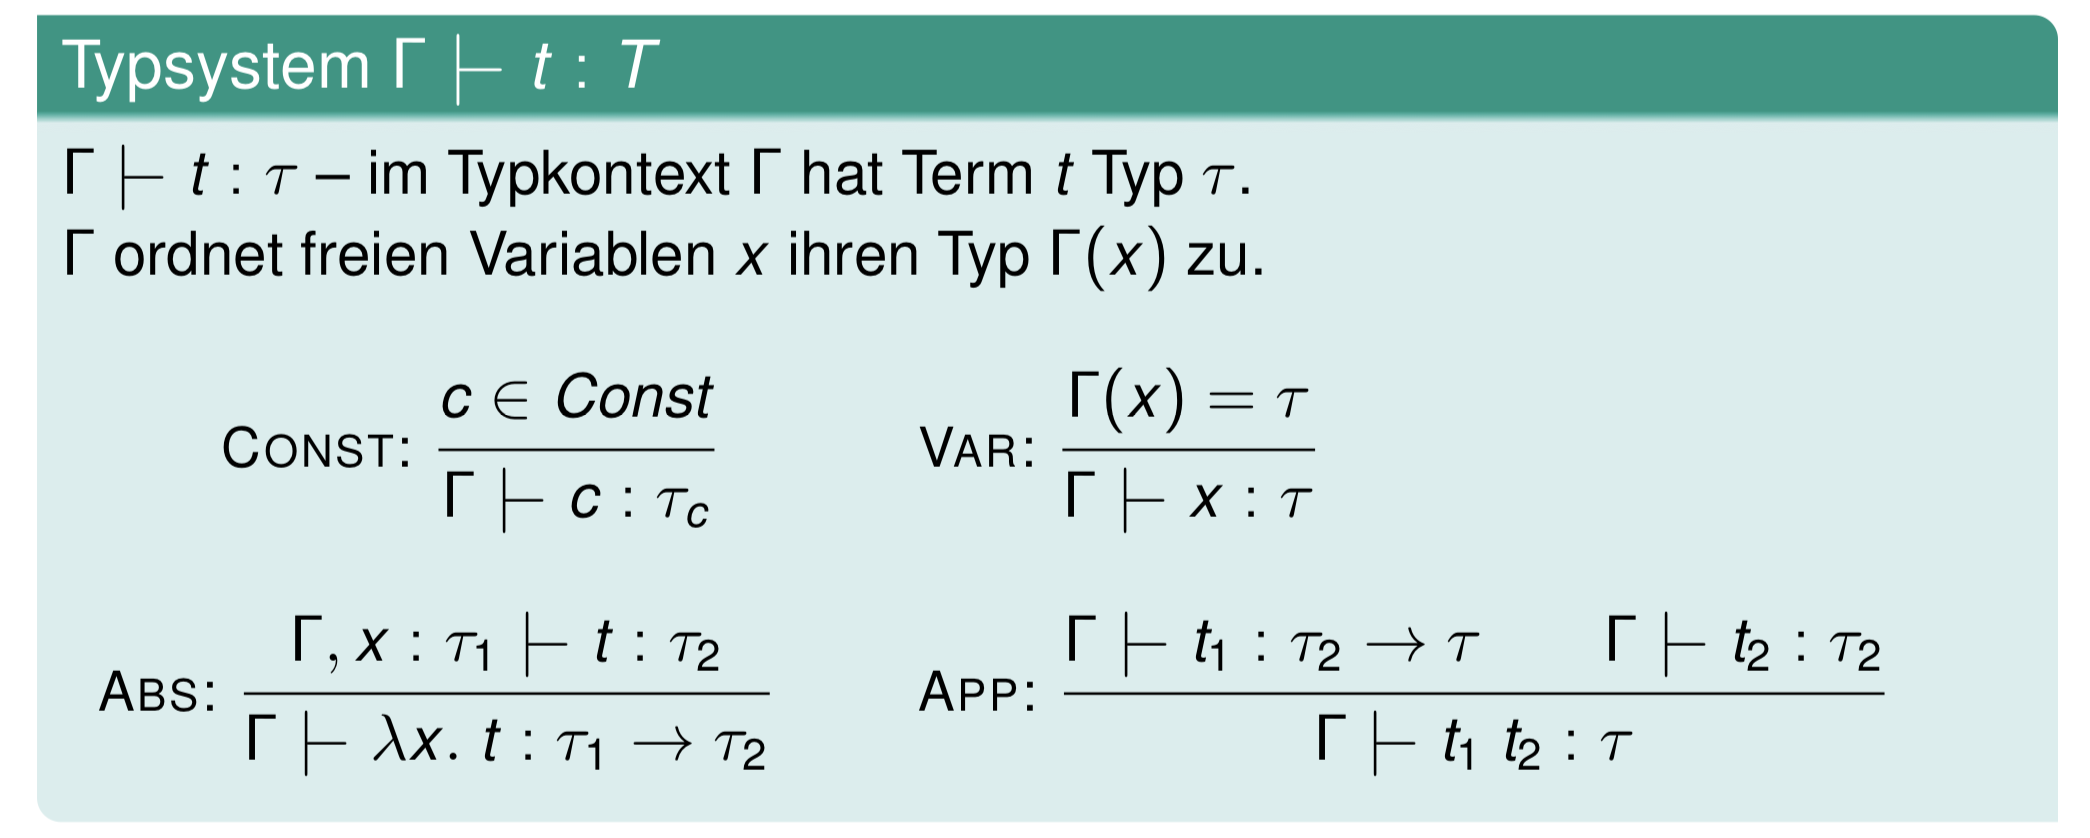
\includegraphics[width=0.75\textwidth]{images/types.png}	
\end{center}
\begin{center}
		
\includegraphics[width=0.75\textwidth]{images/let.png}
\end{center}
Beispiel:\\
\begin{center}
	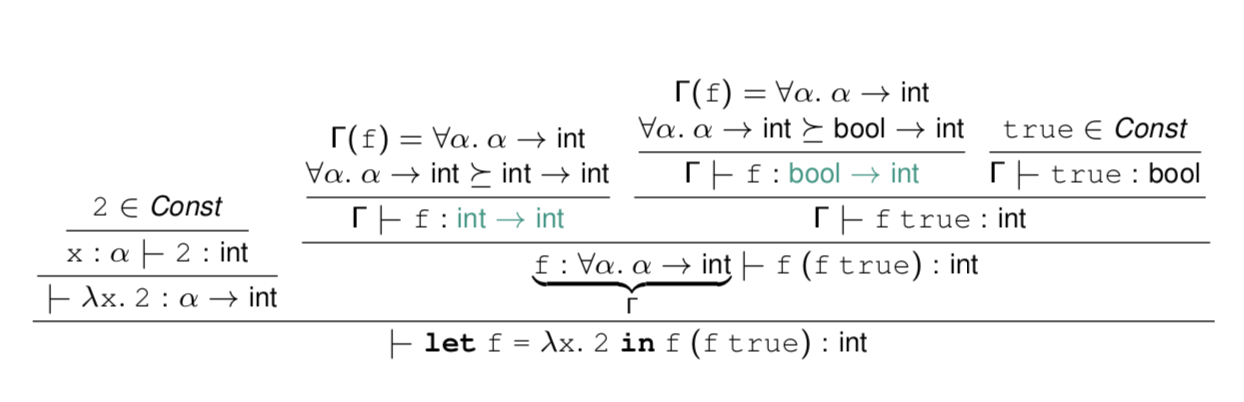
\includegraphics[width=0.75\textwidth]{images/let_ex.png}
\end{center}
\subsubsection{Typisierungsgleichungen}
$$APP \medspace\frac{\Gamma \vdash t_1 : \alpha_2 \medspace\medspace\medspace \Gamma \vdash t_2 : \alpha_3}{\Gamma \vdash t_1 \medspace t_2 : \alpha_1} \rightsquigarrow C_{new} = C \cup \{\alpha_2 = \alpha_3 -> \alpha_1\}$$

$$ABS \medspace\frac{\Gamma, x : \alpha_2 \vdash t : \alpha_3}{\Gamma \vdash \lambda x.t:\alpha_1} \rightsquigarrow C_{new} = C \cup \{\alpha_1 = \alpha_2 -> \alpha_3\}$$

$$VAR \medspace\frac{(x: \alpha_1)(x) = \alpha_2}{\Gamma \vdash x : \alpha_2} \rightsquigarrow C_{new} = C \cup \{\alpha_1 = \alpha_2\}$$

$$Const \medspace\frac{c \in Const}{\Gamma \vdash x : \alpha_1} \rightsquigarrow C_{new} = C \cup \{\alpha_1 = \alpha_c\}$$

\paragraph{Let}
Betrachte:
$$\frac{\Gamma \vdash t_1: \alpha_2 \medspace \Gamma' \vdash t_2: \alpha_3}{\Gamma \vdash \textbf{let} x = t_1 in t_2 : \alpha_1}$$

\begin{enumerate}
	\item Setze $C_0 \coloneqq \{ \alpha_1 = \alpha_3 \}$
	\item Bestimme $C_{let}$ (linker Teilbaum) und $\sigma_{C_{let}}$
	\item Sei $\Gamma_r$ Typannahme rechter Teilbaum, dann ist $\Gamma_r = \Gamma, x: \forall \alpha. ...$
	\item Bestimme $C_{let}' = \{\alpha_i = \sigma_{let}(\alpha_i)\}$
	\item Bestimme constraints rechter Teilbaum $C_r$
	\item Bestimme $\sigma_{(C_0 \cup C_r \cup C_{let}')}$
\end{enumerate}
	% !TeX root = ../propa-cheat-sheet.tex
\section{Haskell Prelude functions}
\subsection{Collections}
\begin{minted}[breaklines]{haskell}
elem :: Eq a => a -> t a -> Bool 
maximum :: forall a. Ord a => t a -> a
minimum :: forall a. Ord a => t a -> a
sum :: Num a => t a -> a
\end{minted}
\subsubsection{Lists}
\begin{minted}[breaklines]{haskell}
map :: (a -> b) -> [a] -> [b]
(++) :: [a] -> [a] -> [a] -- Concat lists
filter :: (a -> Bool) -> [a] -> [a]
head :: [a] -> a -- first element
last :: [a] -> a -- last element
tail :: [a] -> [a] -- everything except the first element
init :: [a] -> [a] -- everything except the last element
null :: Foldable t => t a -> Bool -- Empty check
length :: Foldable t => t a -> Int
reverse :: [a] -> [a]
(!!) :: [a] -> Int -> a -- Index operator
any :: Foldable t => (a -> Bool) -> t a -> Bool -- Test wether any element satisfies a predicate
all :: Foldable t => (a -> Bool) -> t a -> Bool -- Test wether all elements satisfies a predicate
replicate :: Int -> a -> [a] -- replicate n x is a list of length n with x the value of every element.
\end{minted}
\subsubsection{Infinite lists}
\begin{minted}[breaklines]{haskell}
iterate :: (a -> a) -> a -> [a] -- iterate f x == [x, f x, f (f x), ...]
repeat :: a -> [a] -- infinite list from first element: repeat x = [x, x, ...]
cycle :: [a] -> [a] -- turn finite list into circular infinite list
\end{minted}
\subsubsection{Sub-Lists}
\begin{minted}[breaklines]{haskell}
take :: Int -> [a] -> [a]
drop :: Int -> [a] -> [a]
splitAt :: Int -> [a] -> ([a], [a])
takeWhile :: (a -> Bool) -> [a] -> [a]
dropWhile :: (a -> Bool) -> [a] -> [a]
span :: (a -> Bool) -> [a] -> ([a], [a]) -- Tuple longest list of elements satisfying p and second element remainder
break :: (a -> Bool) -> [a] -> ([a], [a]) -- inverse of span, applied to a predicate p and a list xs, returns a tuple where first element is longest prefix (possibly empty) of xs of elements that do not satisfy p and second element is the remainder of the list
zipWith :: (a -> b -> c) -> [a] -> [b] -> [c]
zip = zipWith (,)
unzip :: [(a, b)] -> ([a], [b])
\end{minted}
\subsubsection{Folding}

\textbf{Right to left:}
\begin{minted}[breaklines]{haskell}
foldr :: (a -> b -> b) -> b -> t a -> b
\end{minted}
Usage:
\begin{minted}[breaklines]{haskell}
folded = foldr (\val -> \acc -> newAcc) acc coll
\end{minted}
\textbf{Left to right:} 
\begin{minted}[breaklines]{haskell}
foldl :: (b -> a -> b) -> b -> t a -> b
\end{minted}
Usage:
\begin{minted}[breaklines]{haskell}
folded = foldl (\acc -> \val -> newAcc) acc coll
\end{minted}
\textbf{Bsp.:}
\begin{minted}[breaklines]{haskell}
foldr (+) 0 [1,2,3,4]
\end{minted}
berechnet den Wert (1+(2+(3+(4+0)))) – rechts-geklammert 
\begin{minted}[breaklines]{haskell}
foldl (+) 0 [1,2,3,4]
\end{minted}
den Wert ((((0+1)+2)+3)+4) – links-geklammert\\
\subsubsection{Tuples}
\begin{minted}[breaklines]{haskell}
fst :: (a,b) -> a
snd :: (a,b) -> b
curry :: ((a, b) -> c) -> a -> b -> c
uncurry :: (a -> b -> c) -> (a, b) -> c
\end{minted}
\subsection{Values and numbers}
\begin{minted}[breaklines]{haskell}
succ :: a -> a
pred :: a -> a
even :: Integral a => a -> Bool
odd :: Integral a => a -> Bool
gcd :: Integral a => a -> a -> a
lcm :: Integral a => a -> a -> a
(^) :: (Num a, Integral b) => a -> b -> a 
\end{minted}
\subsubsection{Float}
\begin{minted}[breaklines]{haskell}
isNaN :: a -> Bool
isInfinite :: a -> Bool
\end{minted}
\subsection{Misc}
\subsubsection{IO}
\begin{minted}[breaklines]{haskell}
putStrLn :: String -> IO ()
print :: Show a => a -> IO ()
getLine :: IO String
getChar :: IO Char
\end{minted}
\subsubsection{Maybe}
\begin{minted}[breaklines]{haskell}
data Maybe = Nothing |  Just a
\end{minted}
\begin{minted}[breaklines]{haskell}
maybe :: b -> (a -> b) -> Maybe a -> b
\end{minted}
Usage:
\begin{minted}[breaklines]{haskell}
value = maybe orElse mappingAToB maybe instance
\end{minted}

	\appendix\section{Useful prolog functions}
\subsection{Types}
\begin{minted}[breaklines]{prolog}
atom(X) /** Wahr falls Term ein Atom **/
integer(X) /** Wahr falls Integer **/
var(X) /** Wahr falls freie Variable **/
\end{minted}
\subsection{Listen}
\begin{minted}[breaklines]{prolog}
member(X,L) /** is X in L **/
append(S1,S2,S) /** S1 ++ S2 == S **/
rev(X,Y) /** reverse **/
permute(P,X) /** permutations of P **/
\end{minted}
\subsection{Arithmetic}
\begin{minted}[breaklines]{prolog}
X is 3*A+4 /** nicht rückwärts ausführbar! **/
between(Low,High,Value) /** Integers between limits **/  
\end{minted}
\end{document}
